Android is an open source \gls{os} launched in 2007 and today mainly maintained and developed by Google.
It is based on the Linux kernel and mainly targets touch screen devices such as mobile devices or wearables.
The system is designed to run efficiently on battery powered devices with limited hardware and computational capacity.
Android's main hardware platform is the ARM architecture, known for their low power consumption, but it is designed to run in MIPS and x86 processors as well.
The following will give an overview over the architecture of Android and later a deeper insight in the runtime system of Android.
The architecture of the Android software stack can be seen in figure~\ref{fig:androidArchitecture}.
\newline

\begin{figure}[h]
    \centering
    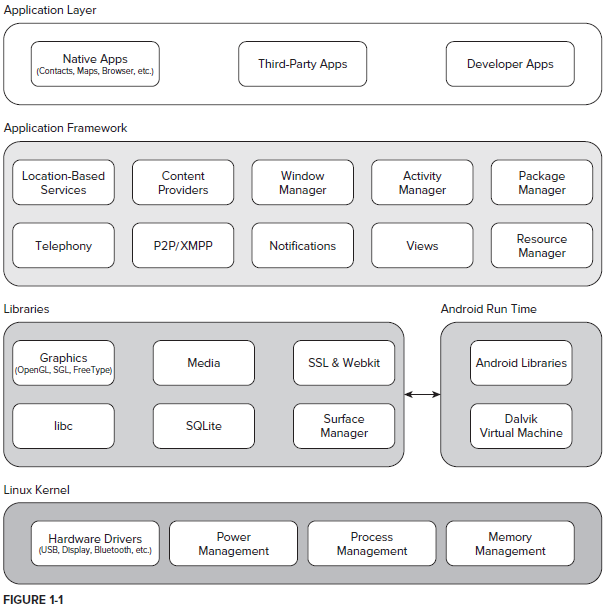
\includegraphics[width=0.8\textwidth]{data/stack.png}
    \caption{Android's architecture \cite{androidStack}}
    \label{fig:androidArchitecture}
\end{figure}

The basis of the system is its kernel.
It is responsible for power and memory management and controls the device drivers.
\newline
The layer above the kernel contains the \gls{art} as well as the native libraries of the system.
\gls{art} and its predecessor, the \gls{dvm}, will be covered in section~\ref{subsection:android-dalvik} and in section~\ref{subsection:android-art}.
\newline
On top of the libraries and the runtime lies the application framework.
This layer provides generic functionality, such as notification support, to applications over Android's \gls{api}.
\newline
The top layer is responsible for the installation and execution of applications.
\newline
Using these layers and abstraction allows software to execute standard Unix commands on the kernel and Android to run on a wide range of devices with different hardware and.
